\chapter{Software Requirement Specification}
\section{Introduction}
\subsection{ Purpose}

[This presents comprehensive description of the intended purpose and environment of KWEST. It fully describes what the KWEST will do and how it will be expected to perform. In addition it also contains non-functional requirements.]

\subsection{ Intended Audience And Reading Suggestion}
The intended audience of this document includes both developers and reviewers of the system.

\subsection{Project Scope}
This project is a virtual file system capable of storing semantics with which it facilitates the finding of relevant information.
\begin{enumerate}
\item  Information is stored in tags, which are extracted from a file's metadata. This
information may be generated implicitly by the system or supplied explicitly by the
user.
\item  The validity of information is based on the users level of organising things.
\item  The system is currently designed to extract metadata from a limited set of popular
file types for audio, video and images and PDF documents.
\item  The modular architecture allows for plugins to be added which can add additional
functionality, and recognition for more file types. This allows the project to be
extended and modified according to the functionality required.
\item  The level of awareness generated by the system is based on the frequency of access
and input provided by the user.
\item  The current implementation is based on the Linux kernel. Future implementations
can be extended to other platforms and devices.
\item  As the system is an virtual entity, it does not need extensive modifications to be
ported to other file systems and operating systems.

\end{enumerate}

\subsection{User Classes And Characteristics} 

The system can be used by three types of users:
\begin{enumerate}
\item General User 

Uses the system without any complex modifications in the system.
\item Advanced User 

Understands the system and creates rules and automation’s based on personal needs.
\item Developer 

Uses the API provided and develops modules that extend the system.
Only advanced users utilise the semantic nature of underlying file system to the fullest.
This does not create any blocks for the general user, who can also use KWEST satisfactorily.
Developers are a different group of users who can extend KWEST through modules. These
modules can modify or define additional behaviour for the system for specific file types.
\end{enumerate}

\subsection{Operating Environment}\begin{enumerate}
\item  KWEST requires FUSE \cite{FUSE} version 2.8.6 and above.

\item KWEST can run on any Linux installation which contains required versions of FUSE.
\item  Furthermore, since kernel version 2.6.14, FUSE has been merged into the
mainstream Linux kernel tree. As a result KWEST can run on any Linux distribution
created from Kernel version 2.6.14 or above.

\item KWEST is a virtual file system mounted to a folder or a loop device.
\item It is the responsibility of the user that mounting and unmounting of the system be
done with standard rules and precaution

\end{enumerate}

\subsection{Design And Implementation Constraints}

Implementation Constraints
\begin{enumerate}
\item KWEST uses FUSE to manage userspace file systems. Hence, access is limited to the
executing userspace for the program.
 \item Since the entire application is executed in userspace only, there cannot be interaction
with the kernel directly.
\item Although KWEST implements a virtual file system which is accessible to all entities,
we have implemented the system with command line as the primary interface. Other
file managers such as Nautilus can only browse but not tag files. This limitation can
be addressed with plugins or additional modules built for the specific file manager.
\item The SQLite database is an integral part of KWEST and is contained in a single file. It
is vital for the system that integrity of the database is maintained.
\end{enumerate}
Design Constraints

\begin{enumerate}

\item Currently, the auto-tagging feature has been limited to common and popular file
types such as audio (mp3, wav, etc.), images (jpeg, png, etc.) and video (mp4, avi,
etc.). This functionality can be extended with modules or through special tools
made specifically for this purpose.

\item The amount of information visible through common file system commands (e.g.
ls - list contents) is a limitation for KWEST. We cannot show tagging information
through these interfaces. Alternate methods for this can be implemented keeping
the end user in mind.
\end{enumerate}


\subsection{ Assumptions And Dependencies}

Assumptions
\begin{enumerate}
\item Users of this software are aware of how semantics are used to categorise
information.
\item Users can recognise or identify appropriate tags in relation to files.
\item It is assumed that the user is well versed in organisation information and uses KWEST
as a tool rather than an assistant.
\item The user has the required privileges / rights to run KWEST and all its operations.
\end{enumerate}
Dependencies

\begin{enumerate}
 \item KWEST uses several external libraries to extract metadata from popular formats for
audio, images etc. TagLib, EXIF etc. which are required at compilation time. These
enable the system to handle metadata extraction for popular file formats.


 \end{enumerate} 


\section{System Features}
\subsection {Tags}
\begin{enumerate}
\item Manual Tagging 

Manual tagging is the basis of semantics in KWEST. The user can assign any tag to the files in KWEST. These tags are then stored internally in a database. The user can create new tags or use tags already defined by the system. Total freedom is given to the user to organise data. Multiple tags can be assigned to the to a single thus allowing its access through multiple locations without duplication of data.
\item Automatic Tagging 

KWEST also features automatic tagging of files. The user can define certain rules under which files will be assigned tags. The system will implement those rules for all files satisfying the defined constraints. This would prevent repetitive tagging operations for the user. 
\item Importing tags 

Certain popular file formats such as mp3, jpeg etc have metadata embedded in them. KWEST supports such popular format and uses this metadata to automatically assign tags to the files. This feature enables the user to collectively classify and store the data under these tags.
\end{enumerate}

\subsection{Database}
\begin{enumerate}
\item Consistency 

KWEST uses an internal database to store and manage data. It is vital that the database always remains consistent. KWEST uses logging mechanisms to ensure that operations on the database always reach an endpoint. 
\item Access 

The database files used by KWEST are not locked down or access restricted. The KWEST API provides facilities that can be used to access the database. However, this feature is made available with the understanding that the integrity of the database will be maintained always.
\end{enumerate}

\subsection{Relation With Existing Data}
\begin{enumerate}
\item Importing semantics 

Users already have certain organisational structures in the way they store data in file systems. KWEST imports these semantics by converting the storage hierarchy to tag-based hierarchy. This allows the entire file system to be imported into KWEST along with the users previous organisation structure. 
\item Files are executable ready 

The files can be directly executed through the virtual file system without making any modification to the files like audio, video files can be played through the virtual system, images can viewed and documents can be opened and read.  
\end{enumerate}

\subsection{Exporting Semantics}
\begin{enumerate}
\item Export file system 

As the entire file system exists as a virtual entity, KWEST provides the export feature. Where the file system can be exported to another system where the data can be imported by another instance of KWEST. 
\item Export tagged files 

It is also possible for the user to export data under certain tags to an external location. The semantic organisation showed by tags is converted to actual directories and files are then copied to these directories. This way the user can export KWEST semantics and data to outside locations.
\end{enumerate}
	
\subsection{Modularity}
\begin{enumerate}
\item Modules As Plugins 

KWEST is an extendable system. It can use external modules to increase functionality or to modify existing operations. Support for using modules is built into KWEST right from the design stage. Additional extraction libraries can be included using the plugin module.
\item Support for developers 

KWEST provides support to developers by providing access to all internal features and database. The API layer allows developers to easily supplement internal operations with their modules.
\end{enumerate}

\section {External Interface Requirements}

\subsection {User Interfaces}
The user can use the system through the command line. The system mounts a virtual file system which the user can use to navigate through. If the file explorer/browser supports virtual file system, the user can use that to navigate through the files. 

\subsection {Hardware Interfaces}
No hardware interfaces used as the file system exists as a virtual entity.

\subsection {Software Interfaces}
\begin{itemize}
\item FUSE\cite{FUSE} \\
KWEST uses FUSE to run the file system code in user space without editing the kernel code.The FUSE module provides only a ``bridge'' to the actual kernel interfaces. Major file system operations are defined by FUSE and forwarded to KWEST for implementation.
\item SQLite\cite{SQLITE} \\
KWEST uses SQLite database to store data. In contrast to other database management systems, SQLite is not a separate process but an integral part of KWEST. Database is accessed and modified for most of the operations performed by KWEST.
\end{itemize}
\subsection {Communication Interfaces}
KWEST can be accessed like any other file system via Command line or file managers like Nautilus, Thunar etc.

\section {Nonfunctional Requirements}

\subsection {Performance Requirements}
\begin {itemize}
\item Response Time \\
The response time for any action on the file system or the database should be reasonable under normal operational circumstances. 
\item Capacity \\
KWEST can be used by any user with sufficient permissions to initialise the filesystem. Subsequent operations like read, write, modify etc. are restricted by user permissions similar to normal file systems.
\item Scalability \\
KWEST provides suggestions and includes automated tagging rules for Audio, Video and Images. It also allows manual tagging of files by the user. Various modules can be further added for recognising and categorising other file types.
\end{itemize}

\subsection {Safety Requirements}
\begin{itemize}
\item Power Failure \\
The system maintains a log file for database. It prevents data corruption by committing data that has been fully written to the log. This should prevent most, if not all, data corruption.
\item Data Loss \\
If any file is accessed which is mentioned in database but deleted from the system then it is removed from the database and appropriate message is displayed to user.
\item Access Rights \\
The system checks if the file tagged is available to user for access. It does not allow files to be included which cannot be access by the user.
\end{itemize}

\subsection {Security Requirements}
KWEST can be used only by a single user with sufficient rights to execute the software. No other user will have permissions to modify tags and files in the system.

\subsection {Software Quality Attributes}
\begin{itemize}
\item Availability \\
The System shall be available from mounting the file system until its unmounted.
\item Updatability \\
The system shall allow for addition or deletion of files under tags.
\item Reliability
\begin{itemize}
\item The system shall save new tags created by active user.
\item The system shall save the file path of an active user to database whenever new files are added to a tag.
\item The system shall maintain a log file which records every operation on database.
\item The system shall modify database whenever tags or files are deleted.
\item The system shall remove file entries from database whenever it is unable to access them.
\end{itemize}
\item Portability \\
The system is implemented on Linux. It is compatible with various other Linux distributions like Ubuntu, Fedora, Red Hat, etc.
\item Testability \\
New modules designed to be added to the system, to identify file types other than audio, video and images must be tested to check if they are compatible with input-output format of the system.
\item Usability \\
The system does not have a large learning curve as the user deals with commands common to all file systems. Documentation provided for the system will include user manuals, developer reference and common FAQ.
\end{itemize}

\section{Other Requirements}
\subsection{Legal Requirements}

All the libraries, programs used in this project are open sourced under GPL. SQLite is a
database which is free to use, distribute or modify. The FUSE kernel module is merged
with the Linux Kernel, which is open sourced and freely available under GPL. There
are no proprietary or closed source products, libraries or interfaces used in this program.
The project KWEST and its subsequent implementations will be open sourced under the
GPL upon completion.

%\newpage
\section {Analysis Model}
\subsection {Data Flow diagram}
\vspace*{1.5cm}
\hspace{6.5cm} \textbf{Level 0} \\


\begin{figure}[H]
\centering
\setlength\fboxsep{0pt}
\setlength\fboxrule{0.5pt}
\fbox{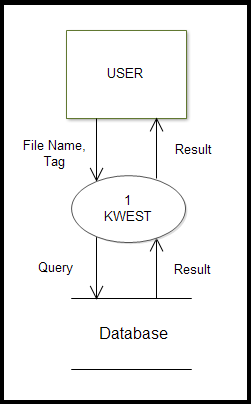
\includegraphics[width=0.5\linewidth]{./diagrams/dfd0.png}}
%\includegraphics[width=0.8\textwidth]{image.png}
\caption{Data flow diagram - Level 0}
\label{fig:dfd0}
\end{figure}

\newpage
\vspace*{2cm}
\hspace{5.5cm} \textbf{Level 1} \\
\begin{figure}[H]
\centering
\setlength\fboxsep{0pt}
\setlength\fboxrule{0.5pt}
\fbox{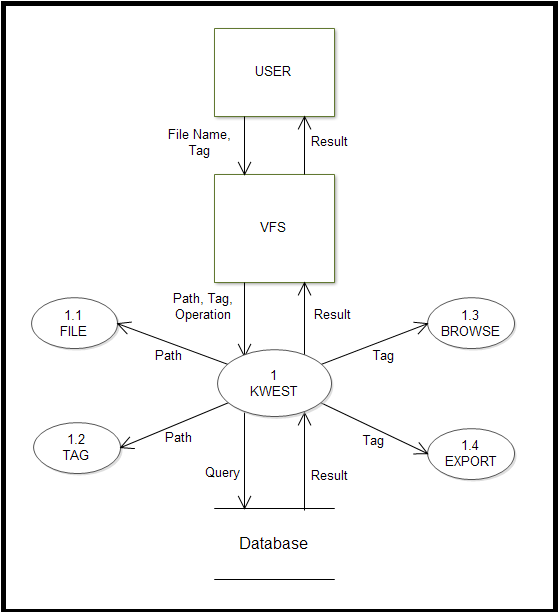
\includegraphics[width=0.9\linewidth]{./diagrams/dfd1.png}}
%\includegraphics[width=0.8\textwidth]{image.png}
\caption{Data flow diagram - Level 1}
\label{fig:dfd1}
\end{figure}

\newpage
\vspace*{2cm}
\hspace{5.5cm} \textbf{Level 2} \\
\begin{figure}[H]
\centering
\setlength\fboxsep{0pt}
\setlength\fboxrule{0.5pt}
\fbox{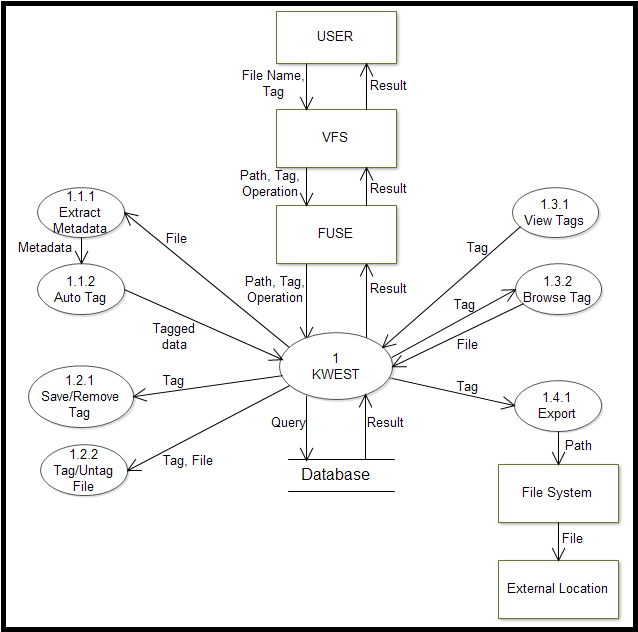
\includegraphics[width=0.9\linewidth]{./diagrams/dfd2.png}}
%\includegraphics[width=0.8\textwidth]{image.png}
\caption{Data flow diagram - Level 2}
\label{fig:dfd2}
\end{figure}

\newpage
\subsection {Entity Relationship diagram}
\begin{figure}[H]
\centering
\setlength\fboxsep{0pt}
\setlength\fboxrule{0.5pt}
\fbox{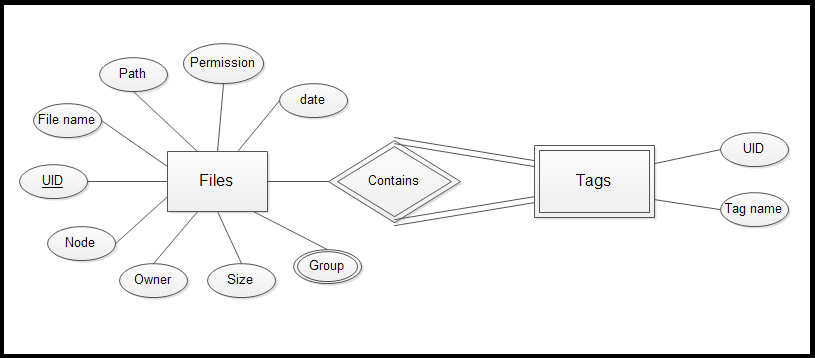
\includegraphics[width=0.8\linewidth]{./diagrams/ER.png}}
%\includegraphics[width=0.8\textwidth]{image.png}
\caption{Entity Relationship diagram}
\label{fig:ERdiag}
\end{figure}



\section{System Implementation Plan}

\subsection*{Phase 1: September 2012 - November 2012}
\begin{table}[h]
\begin{tabular}{|p{7cm}|p{2cm}|p{2cm}|}
\hline
\textbf {Task} & \textbf {Start Date} & \textbf{End Date} \\ \hline
Problem identification & 01/09/12 & 07/09/12 \\ \hline
Information gathering & 08/09/12 & 14/09/12 \\ \hline
Creating problem definition & 15/09/12 & 21/09/12 \\ \hline
Understanding underlying technology & 22/09/12 & 05/10/12 \\ \hline
Analysing problem & 06/10/12 & 12/10/12 \\ \hline
Designing solution & 13/10/12 & 26/10/12 \\ \hline
Refining design & 27/10/12 & 02/11/12 \\ \hline
Creating design report & 03/11/12 & 09/11/12 \\
\hline
\end{tabular}
\caption{Phase 1 Implementation Plan}
\label{tab:P1plan}
\end{table}

\subsection*{Phase 2: December 2012 - March 2013} 
\begin{table}[h]
\begin{tabular}{|p{7cm}|p{2cm}|p{2cm}|}
\hline
\textbf {Task} & \textbf {Start Date} & \textbf{End Date} \\ \hline
Building a stub implementation & 01/12/12 & 14/12/12 \\ \hline
Implement file system operations & 15/12/12 & 28/12/12  \\ \hline
Extract Metadata from files & 28/12/12 & 11/01/13 \\ \hline
Implement modular plugins & 12/01/13 & 25/01/13 \\ \hline
Apply Apriori algorithm to database & 26/01/13 & 08/02/13 \\ \hline
Rigorous testing & 09/02/13 & 22/02/13  \\ \hline
Debugging and refining & 23/02/13 & 08/03/13 \\ \hline
System testing & 09/03/13 & 15/03/13  \\ \hline
Creating implementation report & 16/03/13 & 31/03/13 \\
\hline
\end{tabular}
\caption{Phase 2 Implementation Plan}
\label{tab:P2plan}
\end{table}
